%
%% Kapitel: Stand der Technik
%%======================================================================

\chapter{Auswahl der Entwicklungsumgebung}
\label{cha:Auswahl der Entwicklungsumgebung} \index{Auswahl der Entwicklungsumgebung}

Um Software effizient entwickeln zu k{\"o}nnen ist eine geeignete Programmierumgebung unabdingbar. 
Da nicht jede Entwicklungsumgebung mit ROS kompatibel ist und jede dieser IDEs ihre vor und Nachteile besitzt, wurden Methoden der Entscheidungstheorie angewandt um die bestm{\"o}gliche IDE auszuw{\"a}hlen. Durch die Methode Paarweiser Vergleich wurden die Gewichtungen einzelner Attribute f\"ur eine Nutzweranalyse ermittelt. Es stellte sich heraus das bei der Auswahl einer IDE vorallem wichtig ist, das sie mit dem Betriebssystem Linux kompatibel ist, sie den Code mit CMake buildet und einen guten Debug-Modus besitzt.

\begin{figure}[H]
\begin{center}
  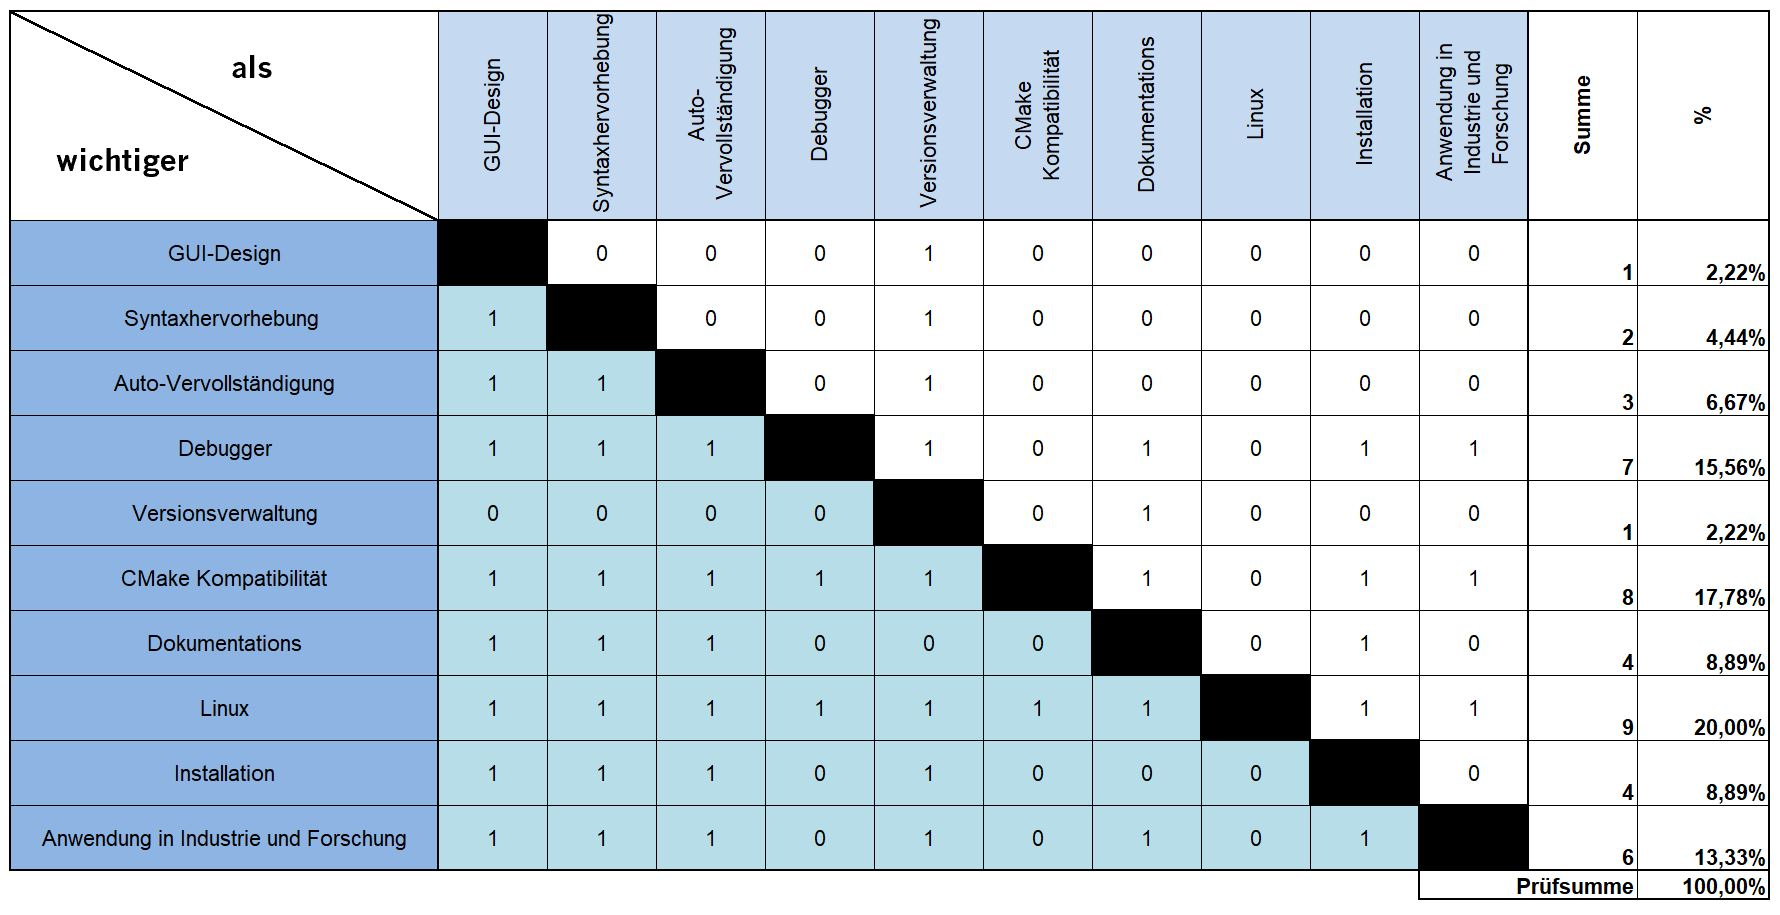
\includegraphics[width=1\textwidth]{/home/tb/Desktop/Master/BA_TB/02_Arbeit_Latex/004_Kapitel3/Bilder/paarweiser_vergleich_ide}% keine extention: wählt jpg für DVI
  \caption[Paarweiser Vergleich der Entwicklungsumgebungen]%
           {\label{fig:Paarweiser Vergleich der Entwicklungsumgebungen}%
           Paarweiser Vergleich wichtiger Attribute einer Entwicklungsumgebung.}
\end{center}
\end{figure}

Durch die Nutzwertanalyse konnten nun die zur Verf\"ugung stehenden Entwicklungsumgebungen verglichen werden. 

\begin{figure}[H]
\begin{center}
  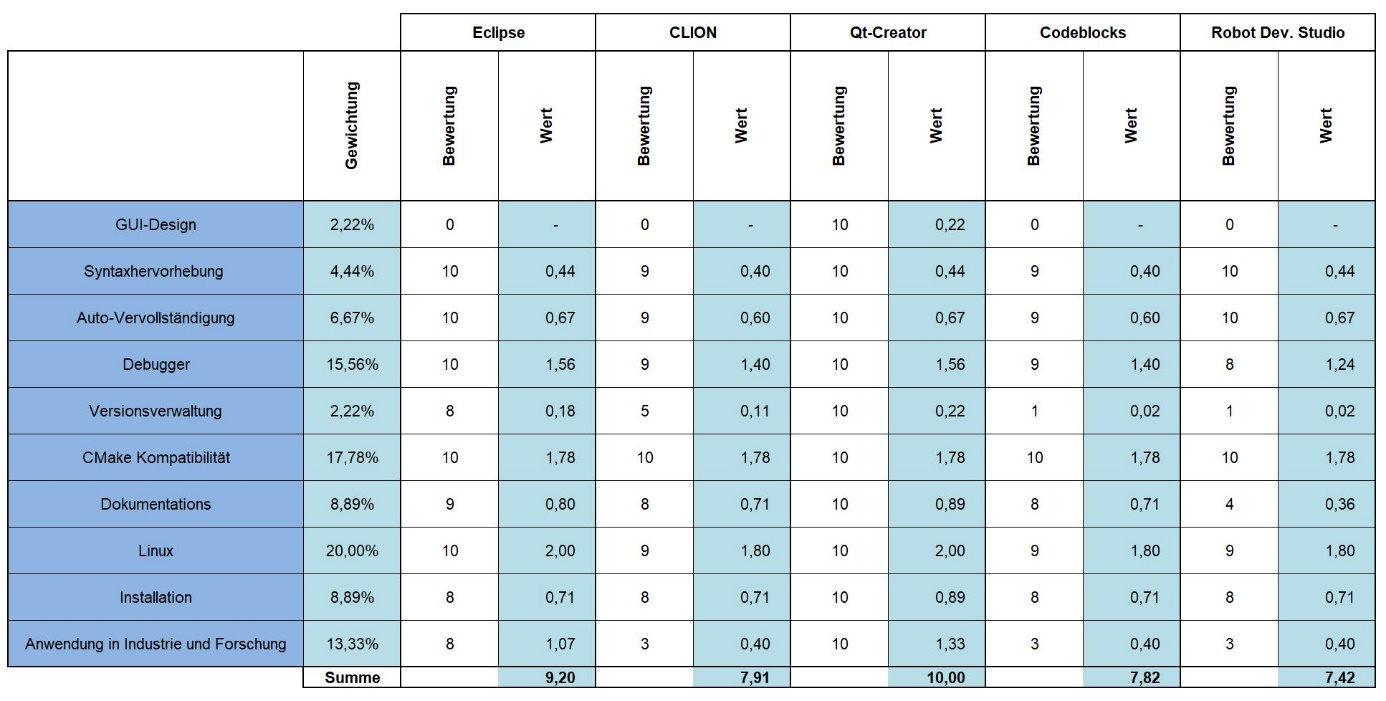
\includegraphics[width=1\textwidth]{/home/tb/Desktop/Master/BA_TB/02_Arbeit_Latex/004_Kapitel3/Bilder/nutzwertanalyse_ide}% keine extention: wählt jpg für DVI
  \caption[Die Auswertung der Nutzwertanalyse der Entwicklungsumgebungen]%
           {\label{fig:Die Auswertung der Nutzwertanalyse der Entwicklungsumgebungen}%
           Die Auswertung der Nutzwertanalyse von verschiedenen Entwicklungsumgebungen.}
\end{center}
\end{figure}


Wie in Abbildung \ref{fig:Die Auswertung der Nutzwertanalyse der Entwicklungsumgebungen} zu sehen ist, ergibt sich durch die Auswertung der Nutzwertanalyse das die Qt-Creator IDE die beste Wahl f{\"u}r die gestellten Anforderungen ist. Vorallem weil sie stark in der Industrie und Forschung angewandt wird, fiel die Wahl auf Qt-Creator. Zudem ist Qt mit zugeh{\"o}rigem ROS-Plugin sehr einfach mit einem Run-Skript zu installieren \cite{rosinstall}. Auch die M{\"o}glichkeit mit Qt Benutzeroberfl{\"a}chen zu entwicklen spricht f\"ur diese IDE.
%https://ros-qtc-plugin.readthedocs.io/en/latest/_source/How-to-Install-Users.html



%\begin{enumerate}

%\item
%\end{enumerate}


